\section*{Desarrollo}
En esta secci\'on se podran observar los pasos para el diseño del filtro y el detalle de los c\'alculos empleados para lograr el comportamiento requerido, junto con las prubeas y respuestas en frecuencia pedidas.\\

%---------------------------------------------------------------%

\subsection*{Problema a resolver}
El filtro a diseñar vino dado por la siguiente ecuaci\'on de transferencia. \\
\begin{equation}
	H(s)=\frac{s^2}{s^2+3510 . s+1.004\times10^7}	
\end{equation}


Esta transferencia es la n\'umero 4, de la lista provista en clase.
Por la forma de la ecuaci\'on, se observa que se trata de un filtro del tipo \textit{Pasa Altos}. Esto es, haciendo limite con $s \rightarrow +\infty$, resulta una amplifiacion de 0\dB \ y se tiene un atenuaci\'on infinita para $s\rightarrow 0$.

\subsection*{Diseño del filtro}
Se identificaron los par\'ametros de la transferencia del filtro a partir de la forma de Bode vista en clase.\\

\begin{equation}
  H(s)=H_0\ \frac{s^2}{s^2 +s \frac{\omega_0}{Q} +\omega_0^2}
\end{equation}
De la consigna se obtiene que la frecuencia de corte es 
$\omega_0=\sqrt{1.004\times10^7}=3169$, por lo que $f_0=\frac{\omega_0}{2\pi}=504\Hz$. Con este dato, encontramos que $Q=\frac{\omega_0}{3510}=0.902$.\\
Ademas, la transferencia tiene un cero doble en $C_0=0$ y polos complejos conjugados en $p_{0,1}= -1755\pm j\ 2638 $. La forma compeja de los polos es coherente al tener $Q>0.5$.
Por ultimo, $H_0 =1$  ya que no hay amplificacion superada la frecuencia de corte.\\
\pagebreak
%---------------------------------------------------------------%

\subsection*{Diagramas de Bode}
Para la transferencia hallada, se realizaron los diagramas de Bode en \texttt{Python} utilizando el m\'odulo \textit{Signal} para procesamiento de señales. Definiendo la transferencia y con la funcio\'on \textit{bode()} se obtuvieron los siguientes gr\'aficos\\
%\pagebreak
\begin{figure}[h]
\begin{center}

\subfloat[Diagrama de Bode de modulo teorico en Python]{
	\begin{minipage}[c]{1\textwidth}
		\centering
		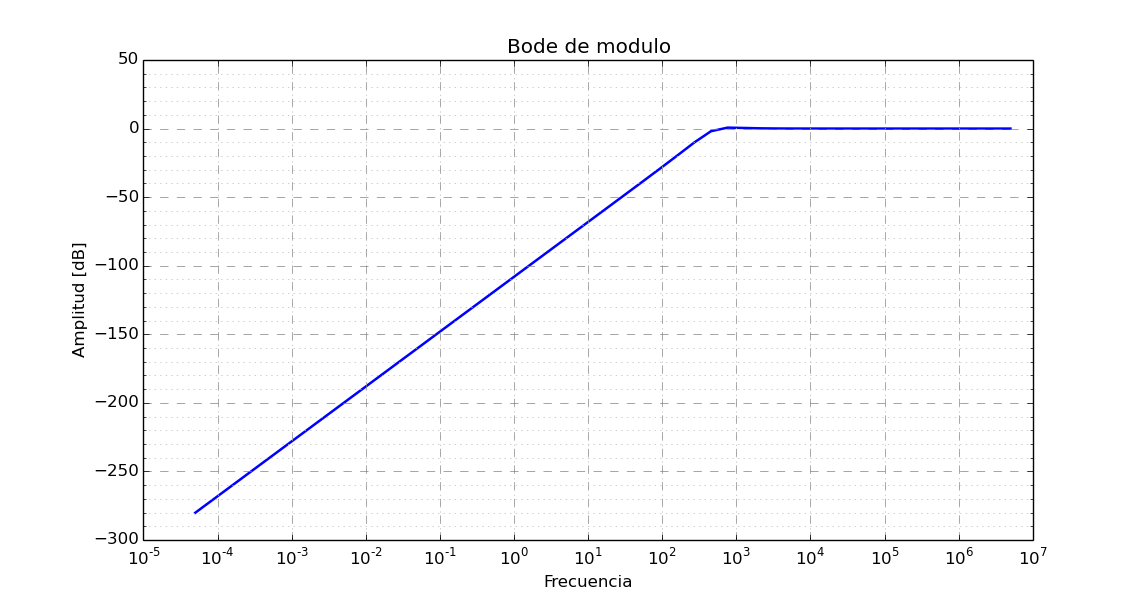
\includegraphics[width=15cm]{imagenes/BodeMod}		%\caption{Diagrama de Bode de modulo teorico en Python}
	\end{minipage}
}
\hfill
\subfloat[Diagrama de Bode de fase en Python]{
\begin{minipage}[c]{1\textwidth}
	\centering
	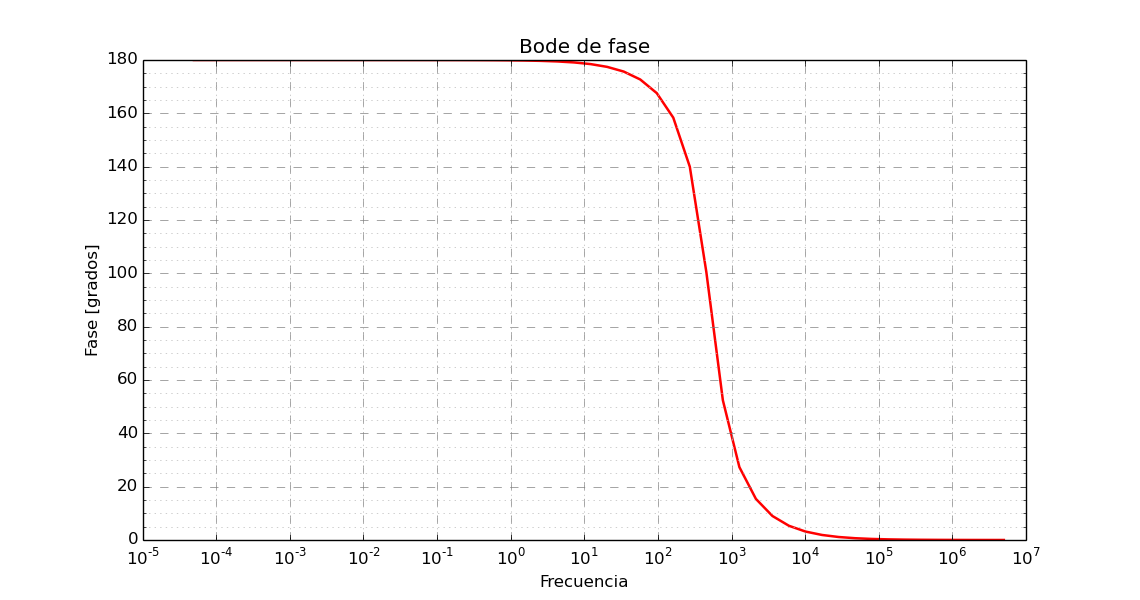
\includegraphics[width=15cm]{imagenes/BodeFase}	%\caption{Diagrama de Bode de fase en Python}
\end{minipage}
}

\end{center}
\end{figure}



Se puede apreciar el comportamiento de \textit{Pasa Altos} y tambien que est\'a aplicado a la frecuencia correcta ($\sim 500\Hz$). Luego viendo el nivel de amplificacion para las altas frecuencias, se observa un nivel de $0 \dB$, lo cu\'al coincide con el esperado.

%---------------------------------------------------------------%
\subsection*{Respuesta del filtro teorico a distintas señales}

Luego del diagrama de Bode, se realizaron graficos donde se muestran qu\'e salida tiene el filtro dada una señal de entrada como: \textit{escal\'on}, \textit{impulso} y \textit{cuadrada}.\\

Para la respuesta a la señal cuadrada, se eligieron tambien,  3 frecuencias acordes, $f_1 = \frac{f_0}{10}=50,4 \Hz$, $f_2 = f_0 = 504\Hz$, $f_3 = 10.f_0= 5,04 \kHz$.
Se lograron los siguientes resultados.\\


\begin{figure}[hbt]
	\centering
	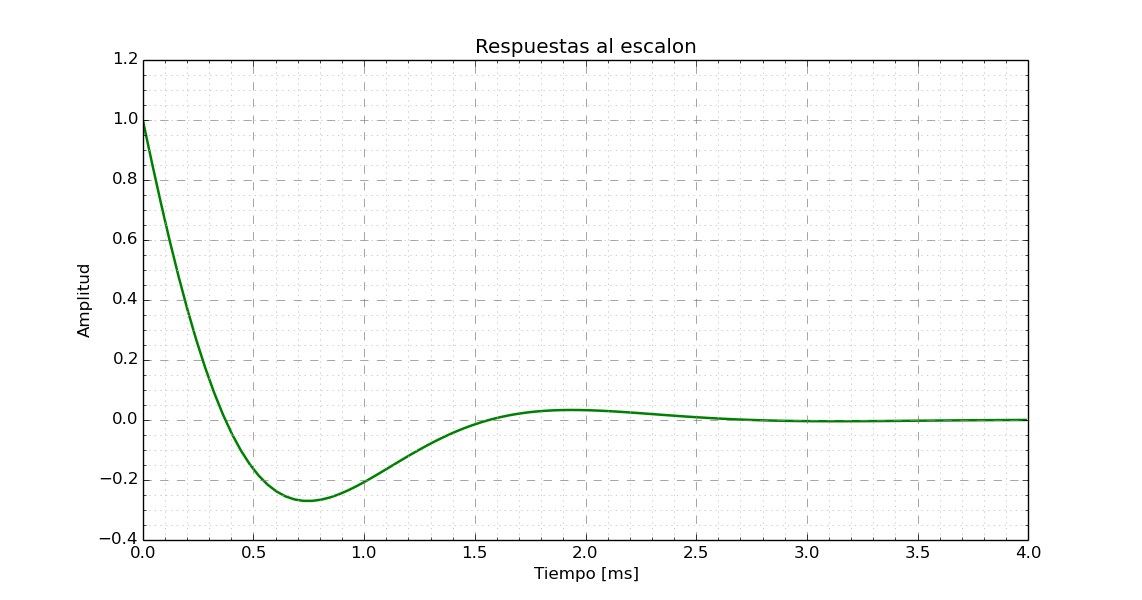
\includegraphics[width=10cm]{imagenes/Step}
	\caption{Respuesta al escal\'on.}
\end{figure}
Se puede observar que se logra un nivel de tensi\'on estable cerca de los $2 \ms$. Es esperable que se vea reflejado en un nivel de $1\V$ al comienzo del escal\'on si consideramos al ascenso a $1\V$  como una señal que contiene a todas las frecuencias. Adem\'as, se ve que el valor al que estabiliza es $0 \V$, que es acorde al comportamiento del filtro si se interpreta a la tensi\'on continua como una señal de frecuencia nula.\\

\begin{figure}[hbt]
	\centering
	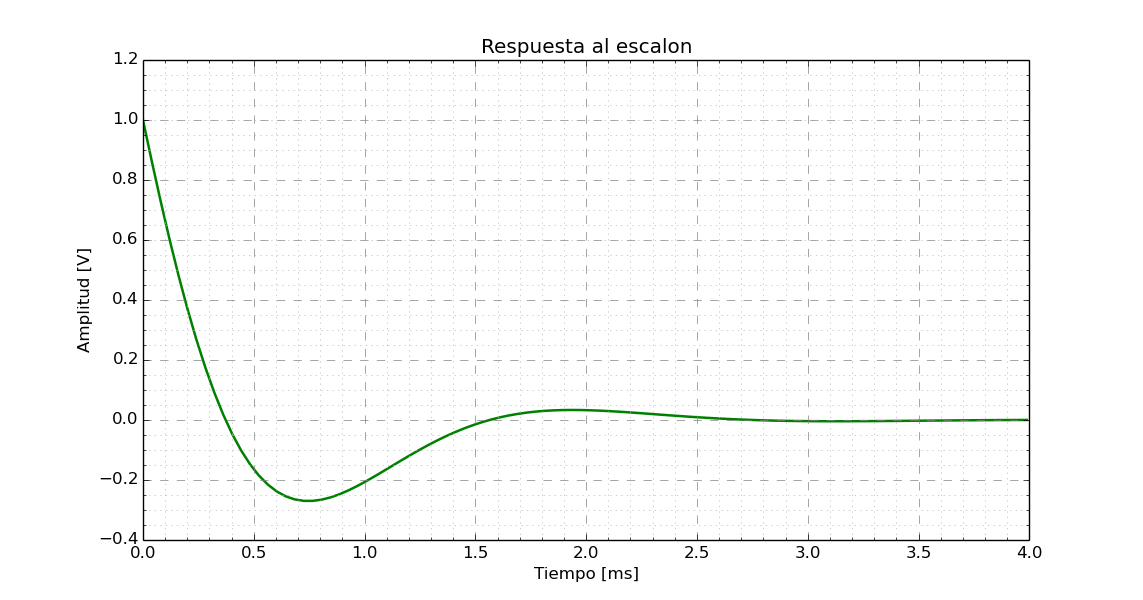
\includegraphics[width=10cm]{imagenes/Impulse}	\caption{Respuesta al impulso.}
\end{figure}
Aqu\'i se observa que existe mucha m\'as variaci\'on de tensi\'on en el transitorio hasta los $0\V$, que se alcanzan en $2 \ms$. Debido a que solo se observa el comportamiento del impuslo desde el $0^+$, este tiene pendiente negativa y por ello el filtro tiene una salida con tensi\'on negativa. \\
Adem\'as, la señal deun impulso se puede considerar como la derivada del escal\'on, resulta entonces razonable con este tipo de sistema (Lineal y temporalmente invariante) que la salida sea la derivada del resultado anterior.

\begin{figure}[H]
	\centering
	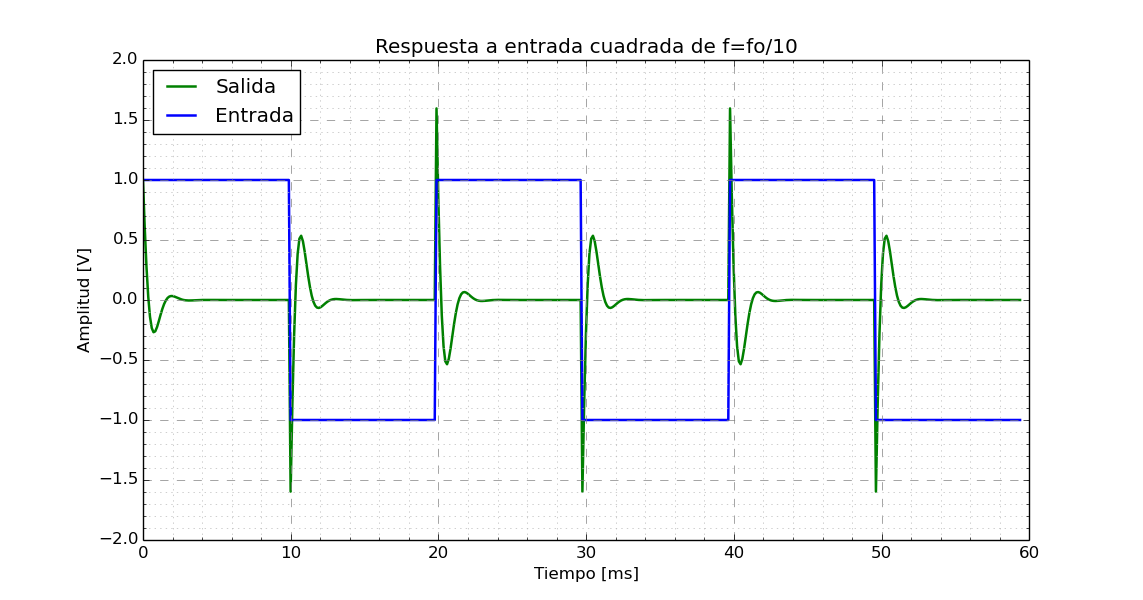
\includegraphics[width=8.3cm]{imagenes/Cuadrada_f:10}	\caption{Respuesta a una señal cuadrada de $50.4\Hz$}	
\end{figure}

Se observa que la señal representada con color verde es la salida  del filtro y de color azul es la señal de entrada. Notar que la salida en general resulta muy atenuada respecto de la entrada,  lo cu\'al es esperado, dada la baja frecuencia de la misma. Asimismo, en los flancos de la cuadrada, se observan grandes oscilaciones en la salida, lo cu\'al es coherente considerando a esos flancos como pequeñas porciones de una señal alta frecuencia.\\

\begin{figure}[hbt]
	\centering
	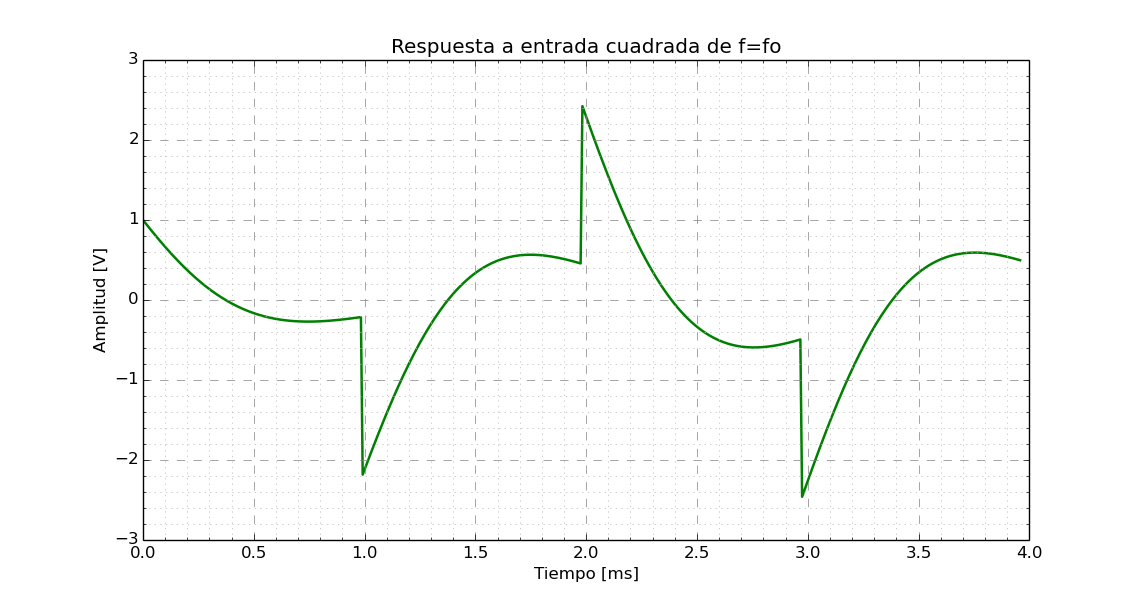
\includegraphics[width=8.3cm]{imagenes/Cuadrada_f}	\caption{Respuesta a una señal cuadrada de $504\Hz$}	
\end{figure}

Aqui se observa que los transitorios de la salida terminan en a tiempo a que se le aplique una tensi\'on identica pero inversa. Se lo puede considerar como un \textit{tren de escalones}. Adem\'as, 
se observa que los picos en los flancos son menores a la salida anterior.\\

\begin{figure}[hbt]
	\centering
	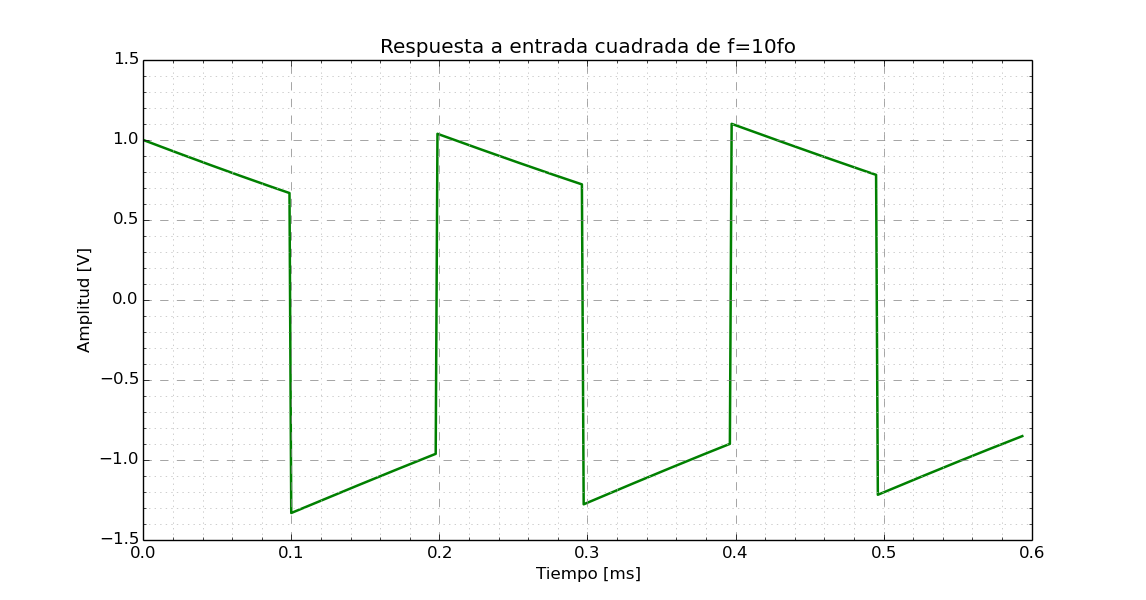
\includegraphics[width=8.3cm]{imagenes/Cuadrada_10f}	\caption{Respuesta a una señal cuadrada de $5.04\kHz$}	
\end{figure}
En esta respuesta, vemos una continuaci\'on de la tendencia a perder atenuaci\'on con el aumento de la frecuencia y asimismo que los picos en los flancos sean cada vez mas bajos, a tal punto que en esta señal son practicamente inexistentes\\

\pagebreak

%---------------------------------------------------------------%

\subsection*{Circuito}
Se propone el siguiente circuito, en base a filtros encntrados en la carpeta y libros:

\begin{figure}[H]
\begin{center}
\begin{circuitikz} [american,scale=0.6,transform shape]
\draw
%capacitores y entrada
(0,0) node[left] {$v_i$} to [short,o-] (1,0)
	to[C,l=$C_1$] (4,0) -- (5,0)
	to[C,l=$C_2$] (7,0)-- (8,0)
;
\draw
%opamp
(9,0.49) node[op amp] (opamp) {}
(opamp) node[] {U1}
(opamp.-) to [short,-o] (7.8,3) -- (10.2,3) to [short,-o]
(opamp.out) to [short,-o] (11,0.49) node[right] {$v_o$}
;
\draw
%R1
(4.5,0) to [short,o-] (4.5,3)
	to[R,l=$R_1$] (7.75,3)
;
\draw
%R2
(7.5,0) to  [short,o-] (7.5,-1)
	to[R,l=$R_2$] (7.5,-4)--(7.5,-5) node[ground]{}; 
;
\end{circuitikz}
\end{center}
\caption{Circuito de filtro Pasa Alto}
\end{figure}	

Aplicando el metodo de \textit{Nodos} se llega a la siguiente transferencia
\begin{equation}
  H(s) = \frac{s^2}{s^2 +s \frac{(C_1 R_1 + C_2 R_1)}{C_1 C_2 R_1 R_2}+\frac{1}{C_1 C_2 R_1 R_2}}
\end{equation}
	
Para elegir los componentes decid\'i fijar $C \defeq C_1 = C_2$ y  dejar $R_1$ y $R_2$ a determinar, dado que por la forma matematica de la transferencia, no es posible dejar ambos valores de resistencias iguales. \\
Resulta entonces la siguiente transferencia, simplificada


\begin{equation}
  H(s) = \frac{s^2}{s^2 +s \frac{2}{C R_2}+\frac{1}{C^2 R_1 R_2}}
\end{equation}

Dadas las ecuaciones
\begin{equation}
	\frac{1}{C^2 R_1 R_2}=1,004\times10^7
\end{equation}
\begin{equation}
	\frac{2}{C R_2}=3510
\end{equation}
Resultan $R_1=5.3 \kohm$ y $R_2=17.27\kohm$,  fijando $C=33\nF$.
Por lo cual, se decidio que para armar el circuito, se utilizarian valores comerciales $R^C_1=4.7\kohm$ y para $R^C_2$ se utilizarian dos resistores de $10\kohm$ en serie, para minimizar el error en la frecuencia de corte y en factor de selectividad.
\pagebreak


%---------------------------------------------------------------%
\subsection*{Circtuio real}
El circuito con los componentes comerciales resulta el siguiente

\begin{figure}[hbt]
\begin{center}
\begin{circuitikz} [american,scale=0.6,transform shape]
\draw
%capacitores y entrada
(0,0) node[left] {$v_i$} to [short,o-] (1,0)
	to[C,l=$ 33\nF $] (4,0) -- (5,0)
	to[C,l=$ 33\nF$] (7,0)-- (8,0)
;
\draw
%opamp
(9,0.49) node[op amp] (opamp) {}
(opamp) node[] {TL084}
(opamp.-) to [short,-o] (7.8,3) -- (10.2,3) to [short,-o]
(opamp.out) to [short,-o] (11,0.49) node[right] {$v_o$}
;
\draw
%R1
(4.5,0) to [short,o-] (4.5,3)
	to[R,l=$4.7\kohm$] (7.75,3)
;
\draw
%R2
(7.5,0) to  [short,o-] (7.5,-1)
	to[R,l=$10\kohm$] (7.5,-3) -- (7.5,-3.5)
	to[R,l=$10\kohm$] (7.5,-5)-- (7.5,-6)
	 node[ground]{}; 
;
\end{circuitikz}
\end{center}
\caption{Circuito de filtro Pasa Alto}
\end{figure}	

Para este circuito, la transferencia resulta

\begin{equation}
	H_R(s)\frac{s^2}{s^2+s \frac{100000}{33}+9768868}
\end{equation}

Con la transferencia determinada, se presentan las diferencias entre los parametros caracteristicos del filtro

\begin{table}[H]
\centering
\begin{tabular}{|c|c|c|c|}
\multicolumn{4}{c}{\textbf{}}\\
\hline
\multicolumn{4}{|c|}{Resultados}\\
\cline{1-4}
Par\'ametro & Ideal & Real &  Error   \\
\hline
$\omega_o$ & 3169 & 3126 &$1.35\%$\\
\hline
$f_0$ & $504\Hz$ & $497\Hz$ & $1.30\%$ \\
\hline
$Q$ & 0.9 & 1.03 & $14.6\%$ \\
\hline

\end{tabular}
\caption{Comparativa entre par\'ametros del circuito ideal y el circuito real}
\label{tabla-datos}
\end{table}

Luego, la forma de la transferencia real produce los siguientes diagramas de Bode

\begin{figure}[h]
	\centering
	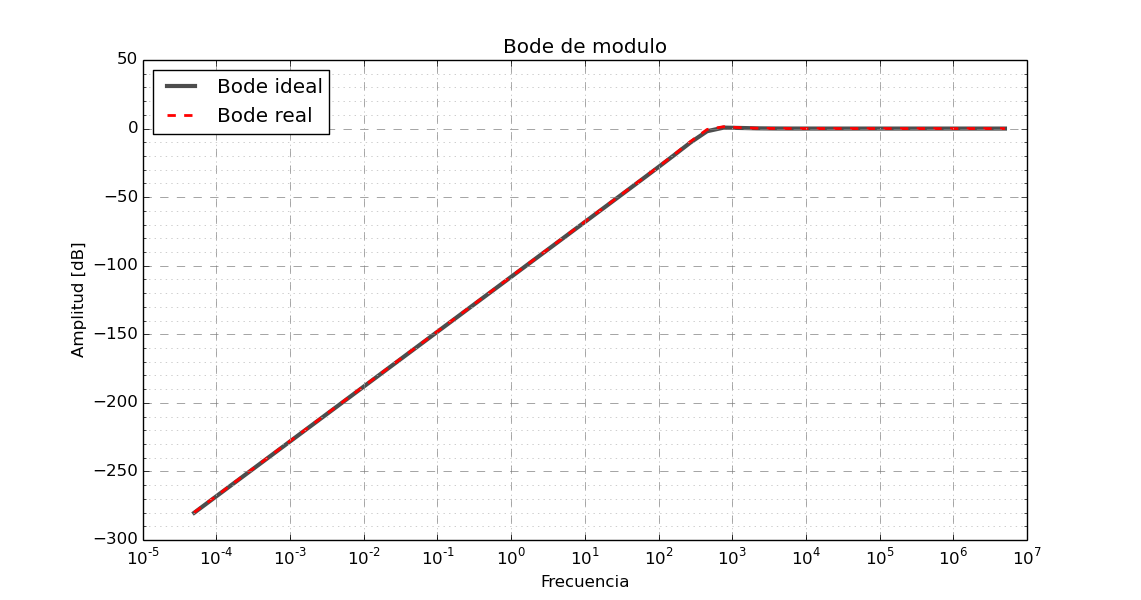
\includegraphics[width=8.3cm]{imagenes/BodeReal}	\caption{Bode de m\'odulo del circuito real, comparado con el ideal}	
\end{figure}
\pagebreak
\begin{figure}[h]
	\centering
	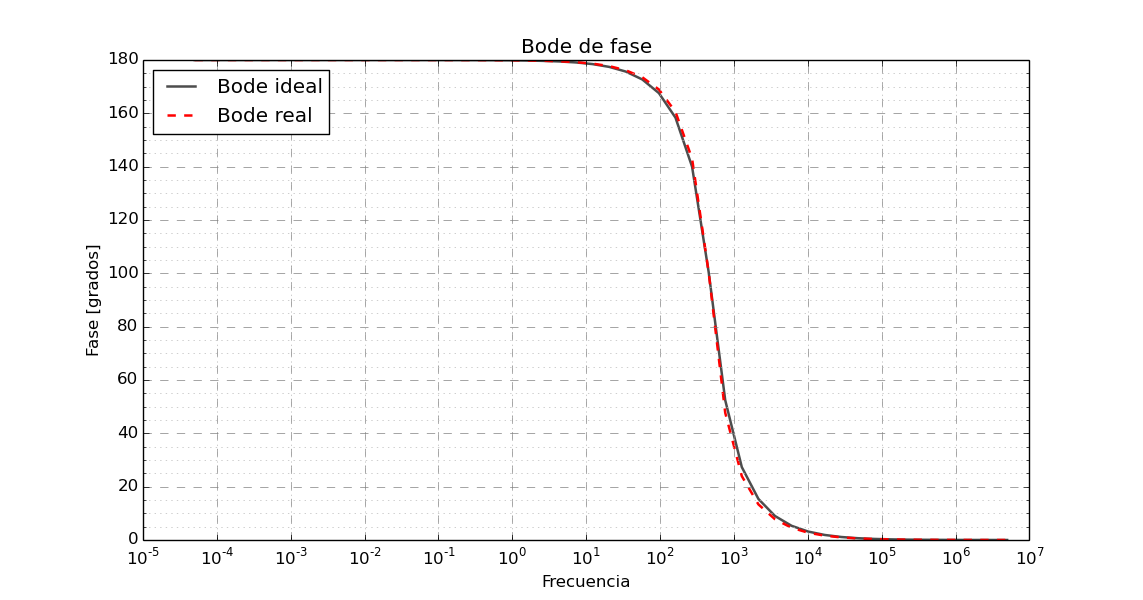
\includegraphics[width=8.3cm]{imagenes/FaseReal}	\caption{Bode de fase del circuito real,comparado con el ideal}	
\end{figure}

De las figuras del \textit{Bode} no se aprecian diferencias significativas. A difenrencia de la respuesta al escal\'on que veremos a continuaci\'on.

\begin{figure}[hbt]
	\centering
	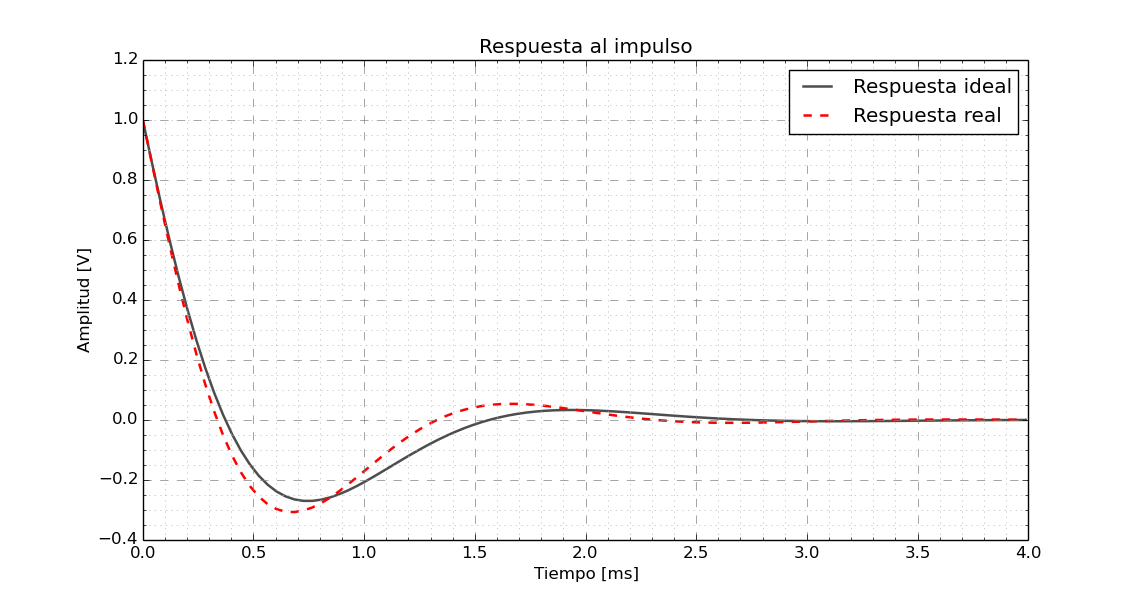
\includegraphics[width=8.3cm]{imagenes/StepReal}
	\caption{Respuesta al escal\'on del circuito real, comparado con el circuito ideal}	
\end{figure}
Aqui las diferencias entre el filtro real y el ideal son mas aparentes, esta diferencia en la forma se corresponde con el aumento en el factor de selectividad $Q$, m\'as que en la diferencia en la frecuencia de corte. Estos es, el fin del transitorio es pr\'acticamente el mismo instante, mientras que los extremos de las curvas mas pronunciados son caracteristicos alaumentar $Q$.
 

%---------------------------------------------------------------%

\subsection*{Simulaci\'on}
	Para verificar que el funcionamiento del circuito sea cerca del esperado, se utiliz\'o el software de simulaci\'on \textit{LTSpice} con los componentes de valores comerciales. Se utiliz\'o el siguiente circuito.\\
	
		
\begin{figure}[hbt]
	\centering
	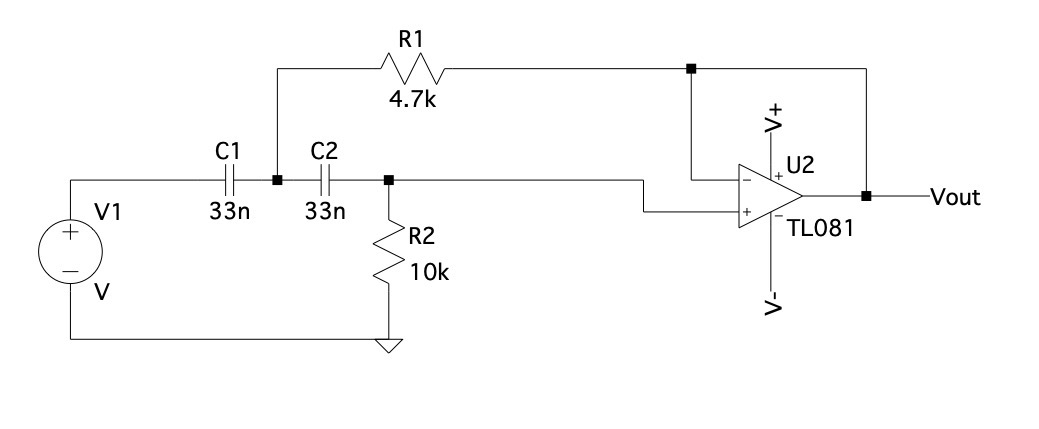
\includegraphics[width=10cm]{imagenes/Simulacion}
	\caption{Diagrama \textit{Bode} del circuito simulado}
\end{figure}
	
\pagebreak	
\begin{figure}[hbt]
	\centering
	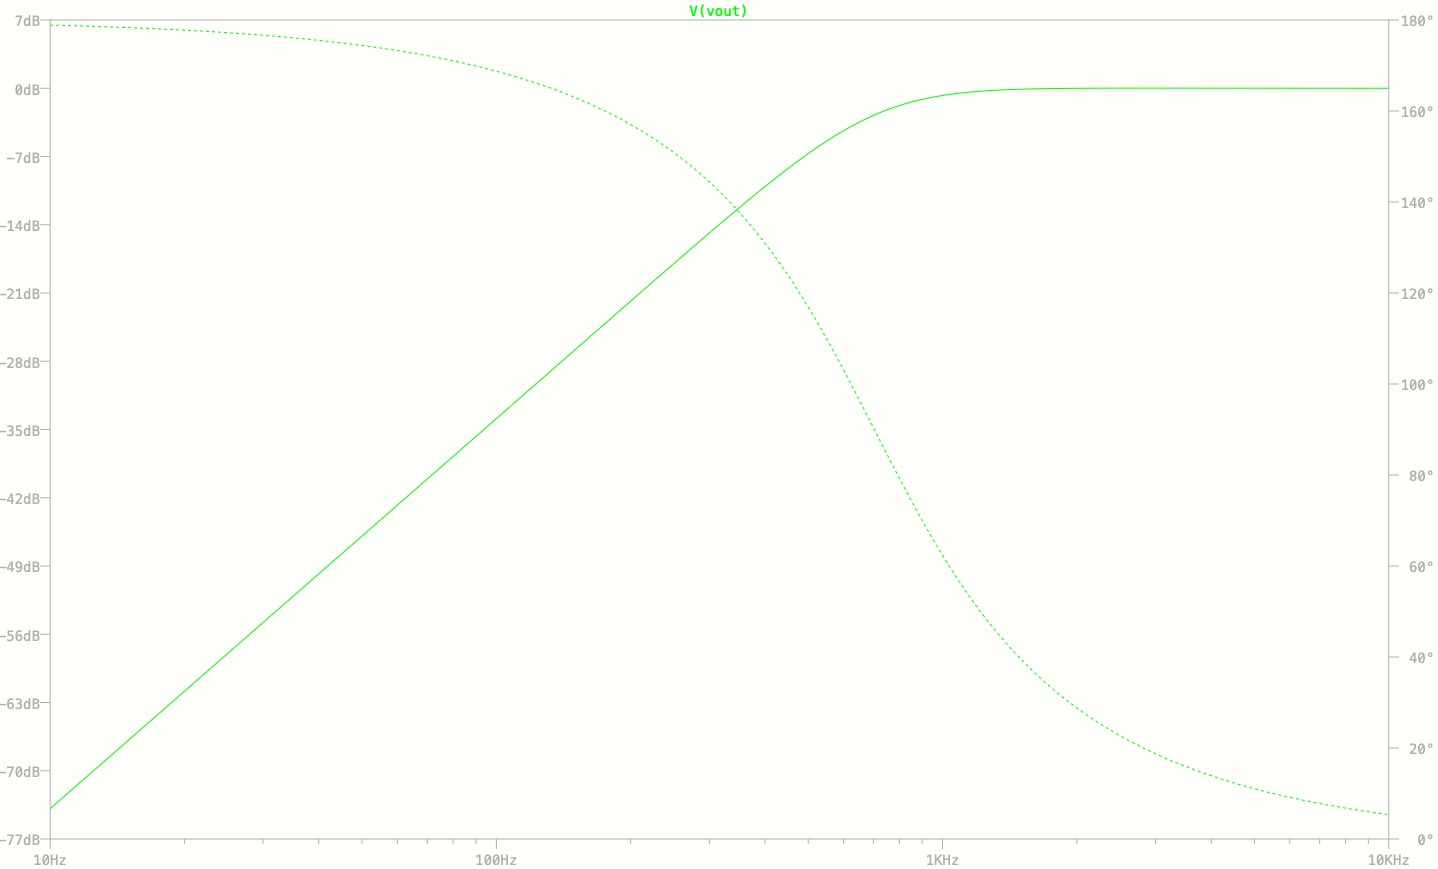
\includegraphics[width=10cm]{imagenes/BodeSimulacion}
	\caption{Diagrama \textit{Bode} del circuito simulado}
\end{figure}

	
Se utiliz\'o la directiva \texttt{.ac dec 100 1 1000000 } para
variar la  frecuencia de la fuente de entrada \texttt{ Vin } desde  $1 \si{\hertz}$ hasta $100 \kHz$. Luego se import\'o la biblioteca \textit{TL081} para el operacional. Produciendo este diagrama que resulta ser coherente con lo estudiado analiticamente.
Luego, seguir\'an pruebas de respuesta en funci\'on de varias de las mismas señales que ya se estudiaron.

\begin{figure}[hbt]
\begin{centering}

	\begin{minipage}[b]{.4\linewidth}
	\centering
	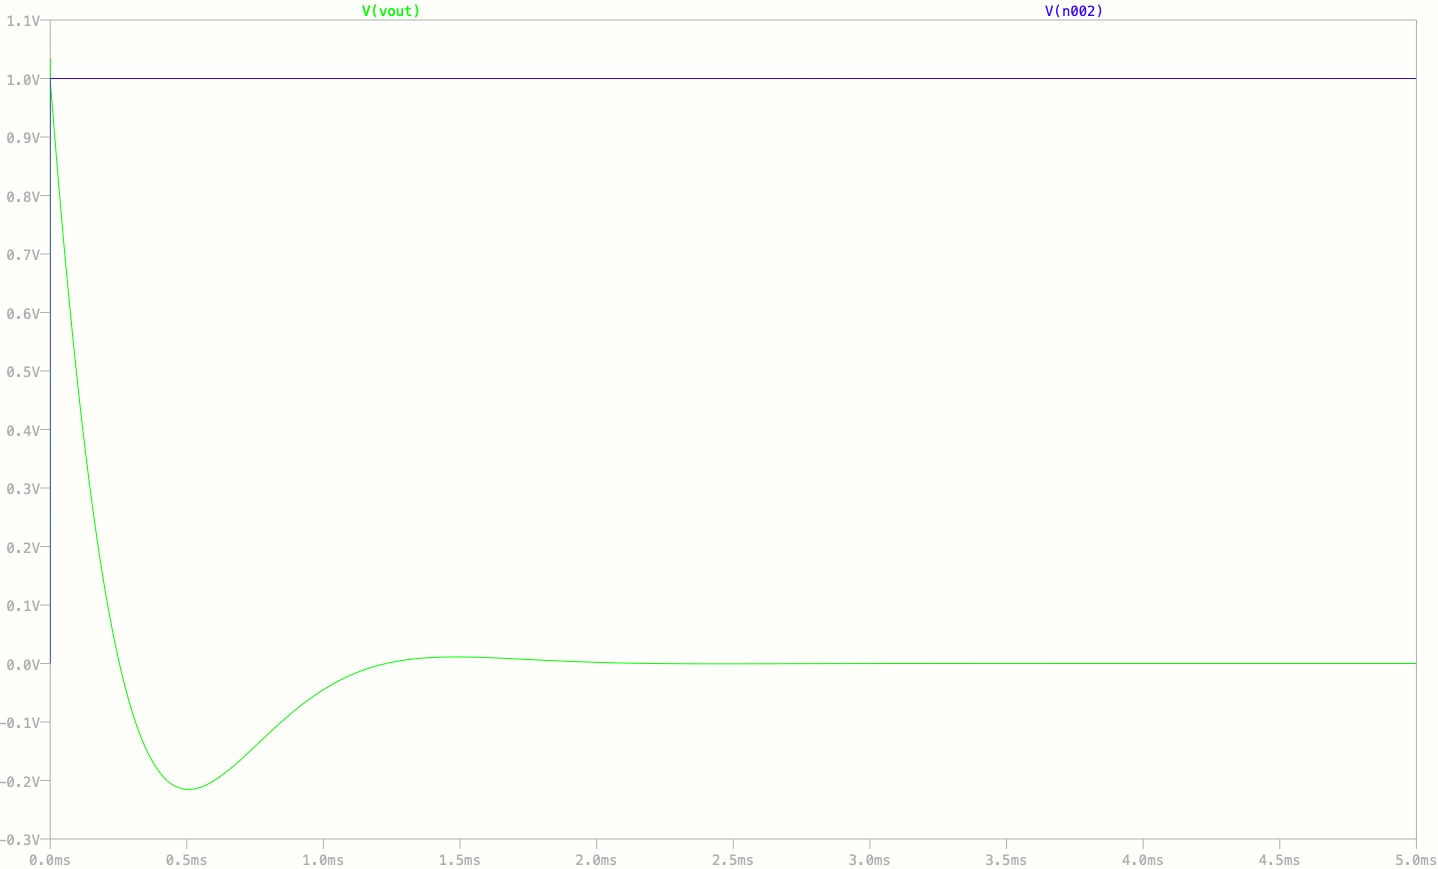
\includegraphics[width=1.1\linewidth]{imagenes/StepSimulacion}
	\caption{Respuesta al escal\'on del circuito simulado}
	\end{minipage}
	\hfill
	\begin{minipage}[b]{.4\linewidth}
	\centering
	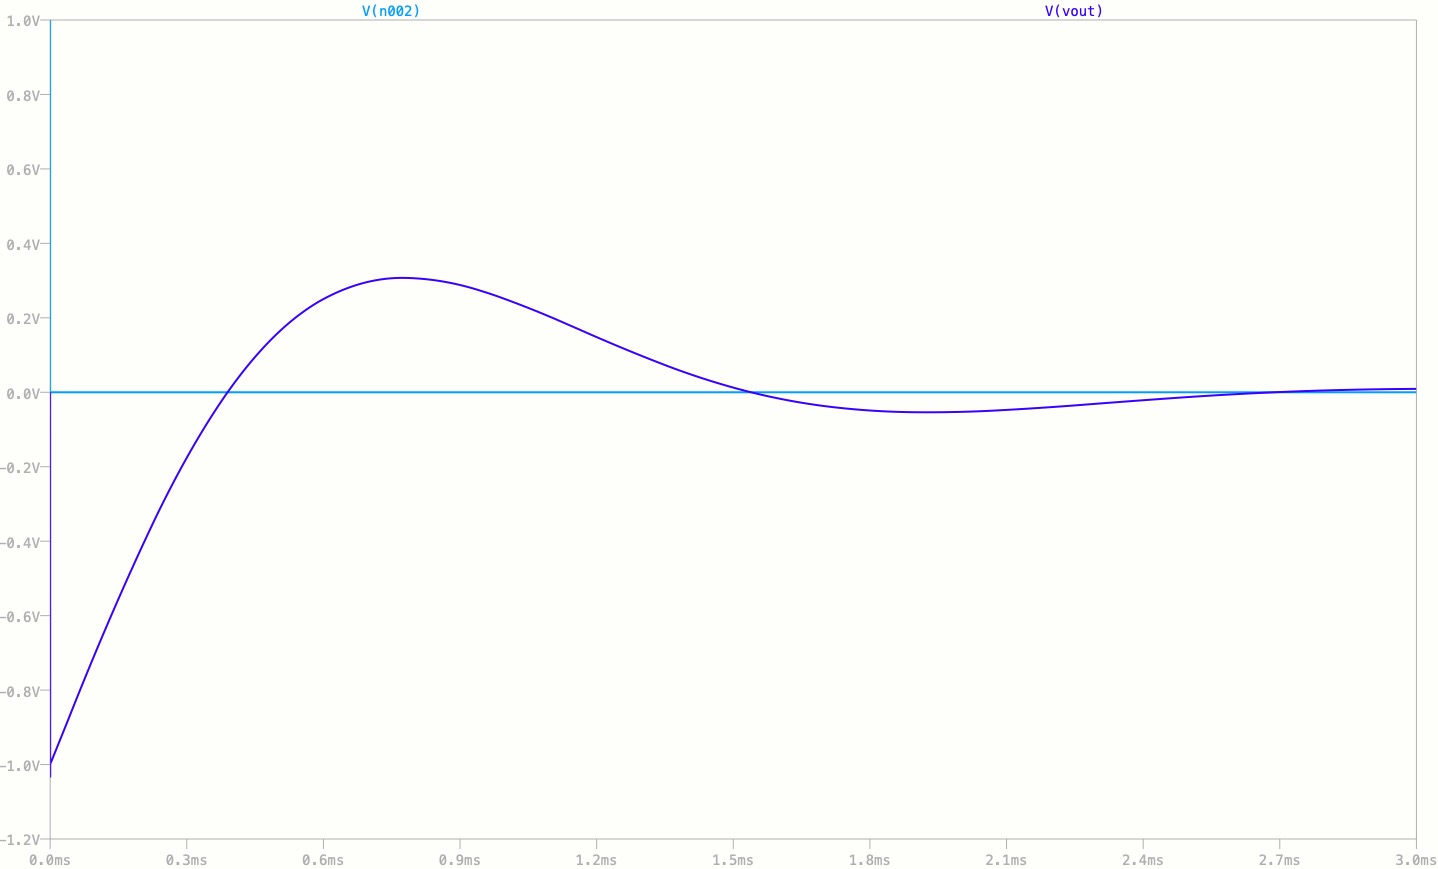
\includegraphics[width=1.1\linewidth]{imagenes/ImpulseSimulacion}
	\caption{Respuesta al impulso del circuito simulado}
	\end{minipage}
\end{centering}
\end{figure}


Estas respuestas se corresponden con los resultados hallados anteriormente, encontrando diferencias en los niveles de tensi\'on. Siendo la curva azul, la  que representa la entrada y la curva verde la que representa la salida.

\begin{figure}[H]
\begin{centering}

	\begin{minipage}[b]{.4\linewidth}
	\centering
	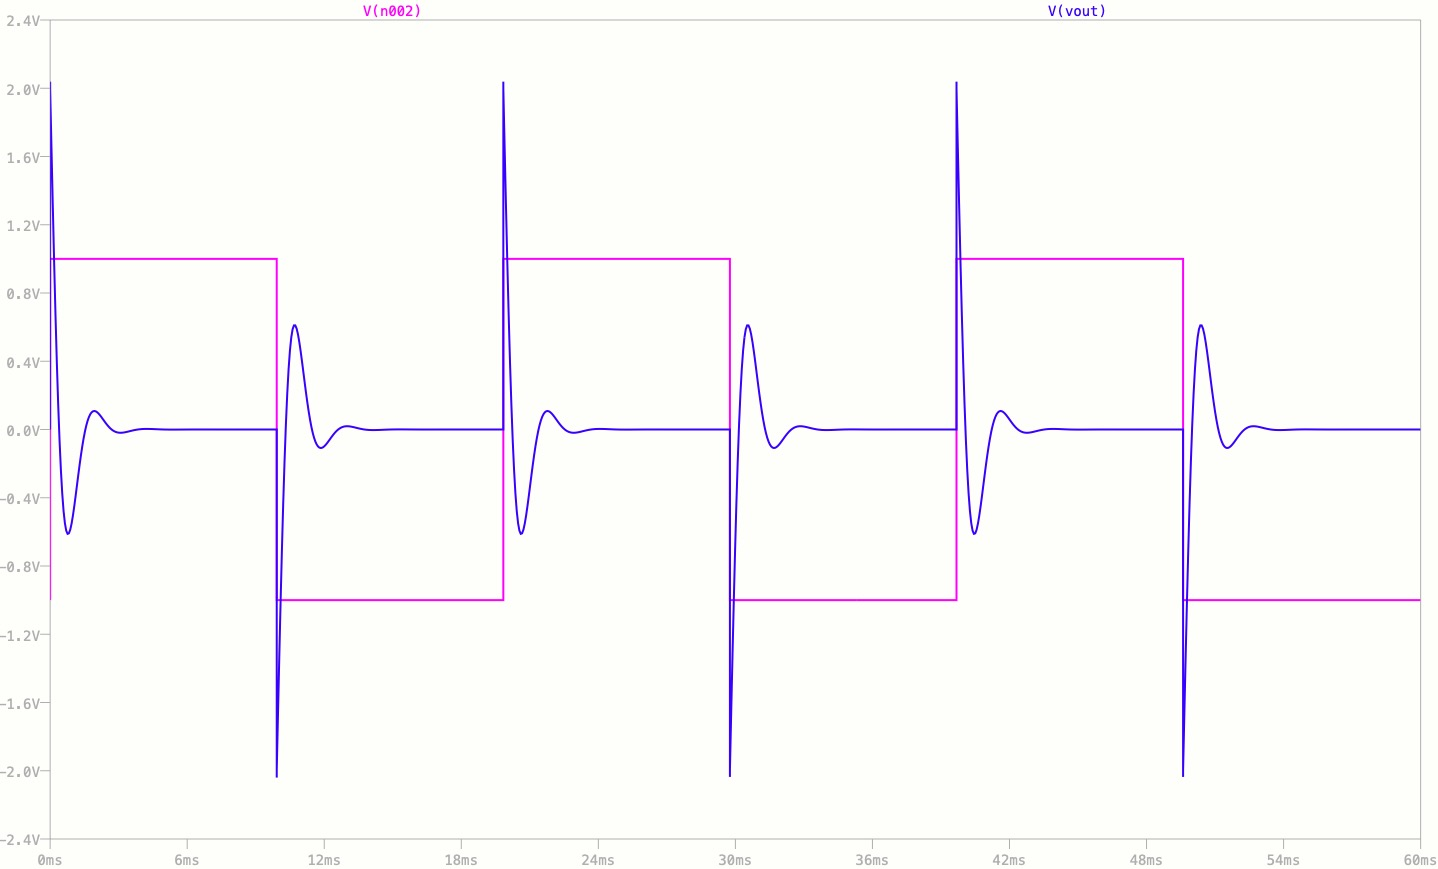
\includegraphics[width=1.1\linewidth]{imagenes/SimCuadrada_f:10}
	\caption{Respuesta a señal cuadrada de $f=\frac{f_0}{10}$ del circuito simulado}
	\end{minipage}
	\hfill
	\begin{minipage}[b]{.4\linewidth}
	\centering
	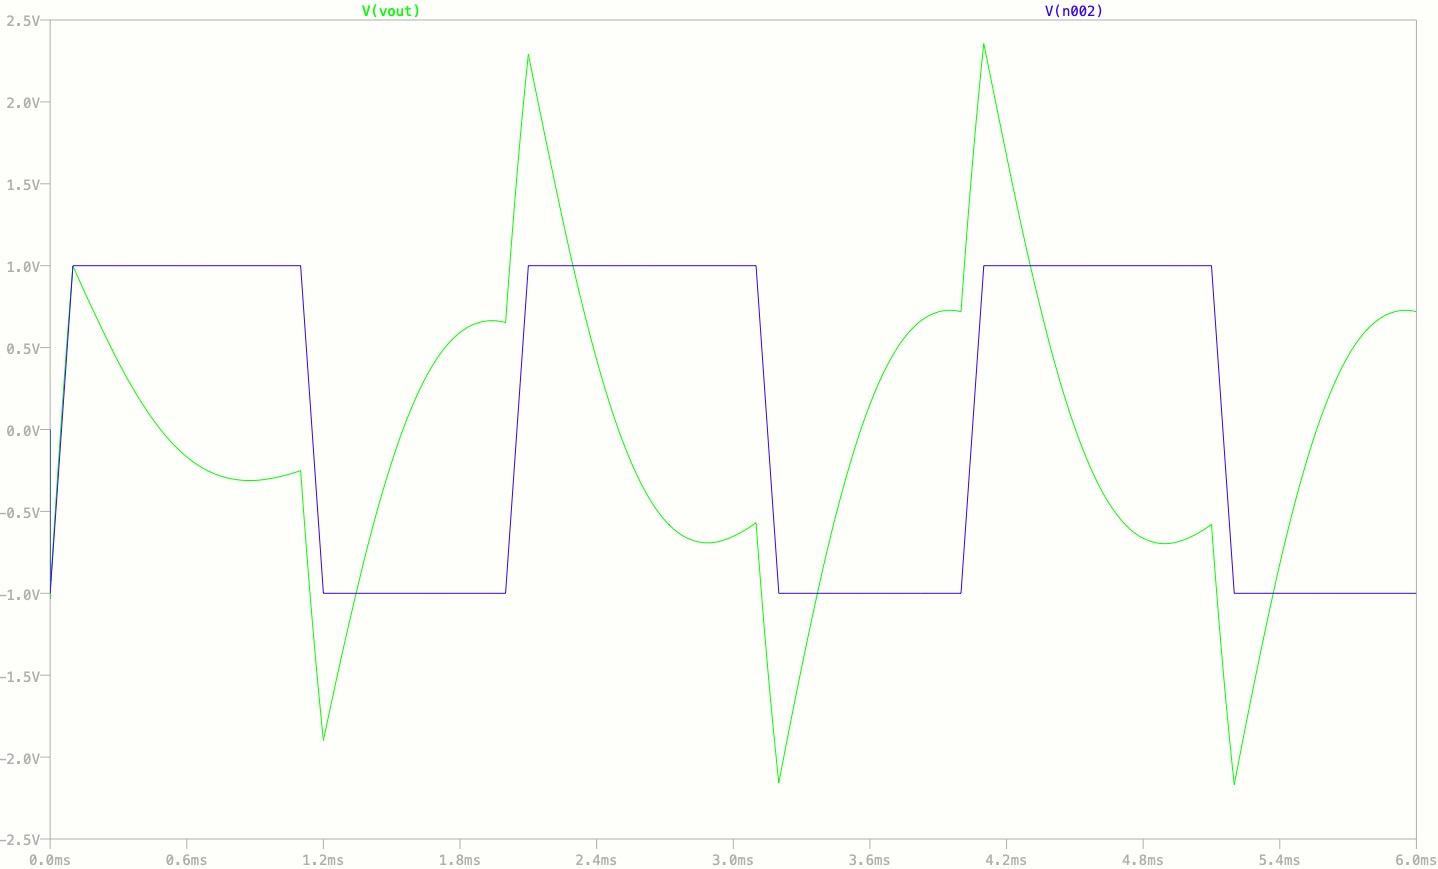
\includegraphics[width=1.1\linewidth]{imagenes/SimCuadrada_f}
	\caption{Respuesta a señal cuadrada de $f=f_0$ del circuito simulado}
	\end{minipage}
\end{centering}
\pagebreak
\end{figure}
\begin{centering}
\begin{figure}[H]
	\centering	
	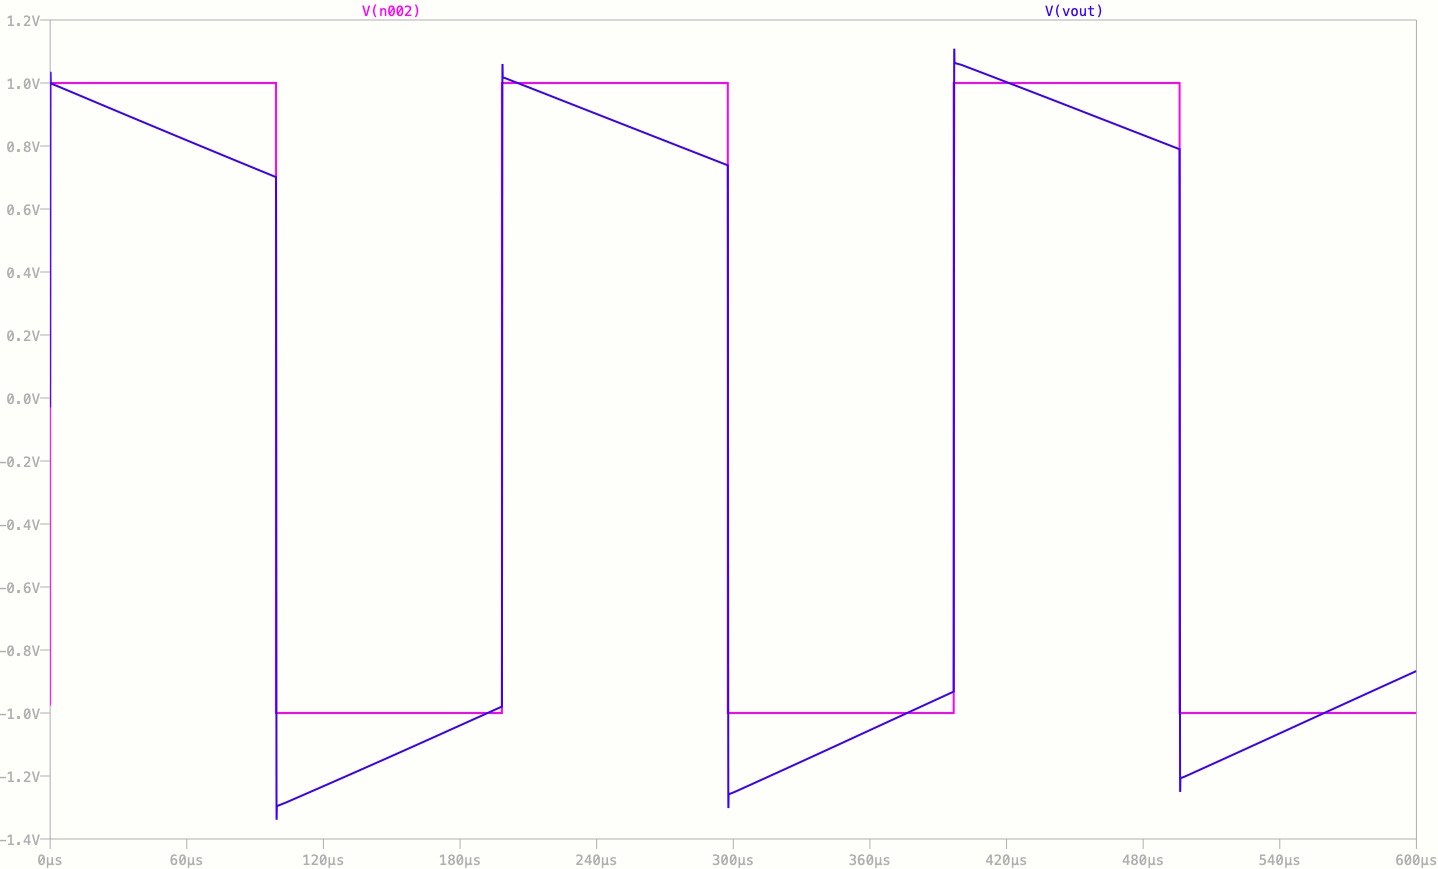
\includegraphics[width=0.4\textwidth]{imagenes/SimCuadrada_10f}	\caption{Respuesta a señal cuadrada de $f=10.f_0$ del circuito simulado}
\end{figure}
\end{centering}
Las respuestas a las señales cuadradas continuan comportandose similar al estudio anal\'itico, aunque existen diferencias en los niveles de tensi\'on que toman las señales.

%---------------------------------------------------------------%
\subsection*{Mediciones}

Se realizazron mediciones sobre el filtro utilizando una fuentes de alimentaci\'on externa, generador de funciones y un osciloscopio. Las primeras mediciones realizadas constaron de visualizar en un osciloscopio los distintos niveles de amplificaci\'on dada una frecuencia de una señal senoidal, se realiz\'o una tabla con frecuencias desde $\frac{f_0}{10}=50.4\Hz$ hasta $10 f_0=5040\Hz$ en pasos de un tercio de octava, con la excepci\'on de los valores cercanos a la frecuencia de corte. All\'i se tomaron 10 puntos entre el tercio de octava anterior y el siguiente a la frecuencia de corte. Esto se realizo para tener un gr\'afico con mayor visibilidad del efecto del factor de selectividad $Q$ alrededor de la frecuencia de corte.\\
El banco de medici\'on para esta y las siguientes mediciones, fue el que se presenta en la siguiente imagen.

\begin{centering}
\begin{figure}[h]
	\centering
	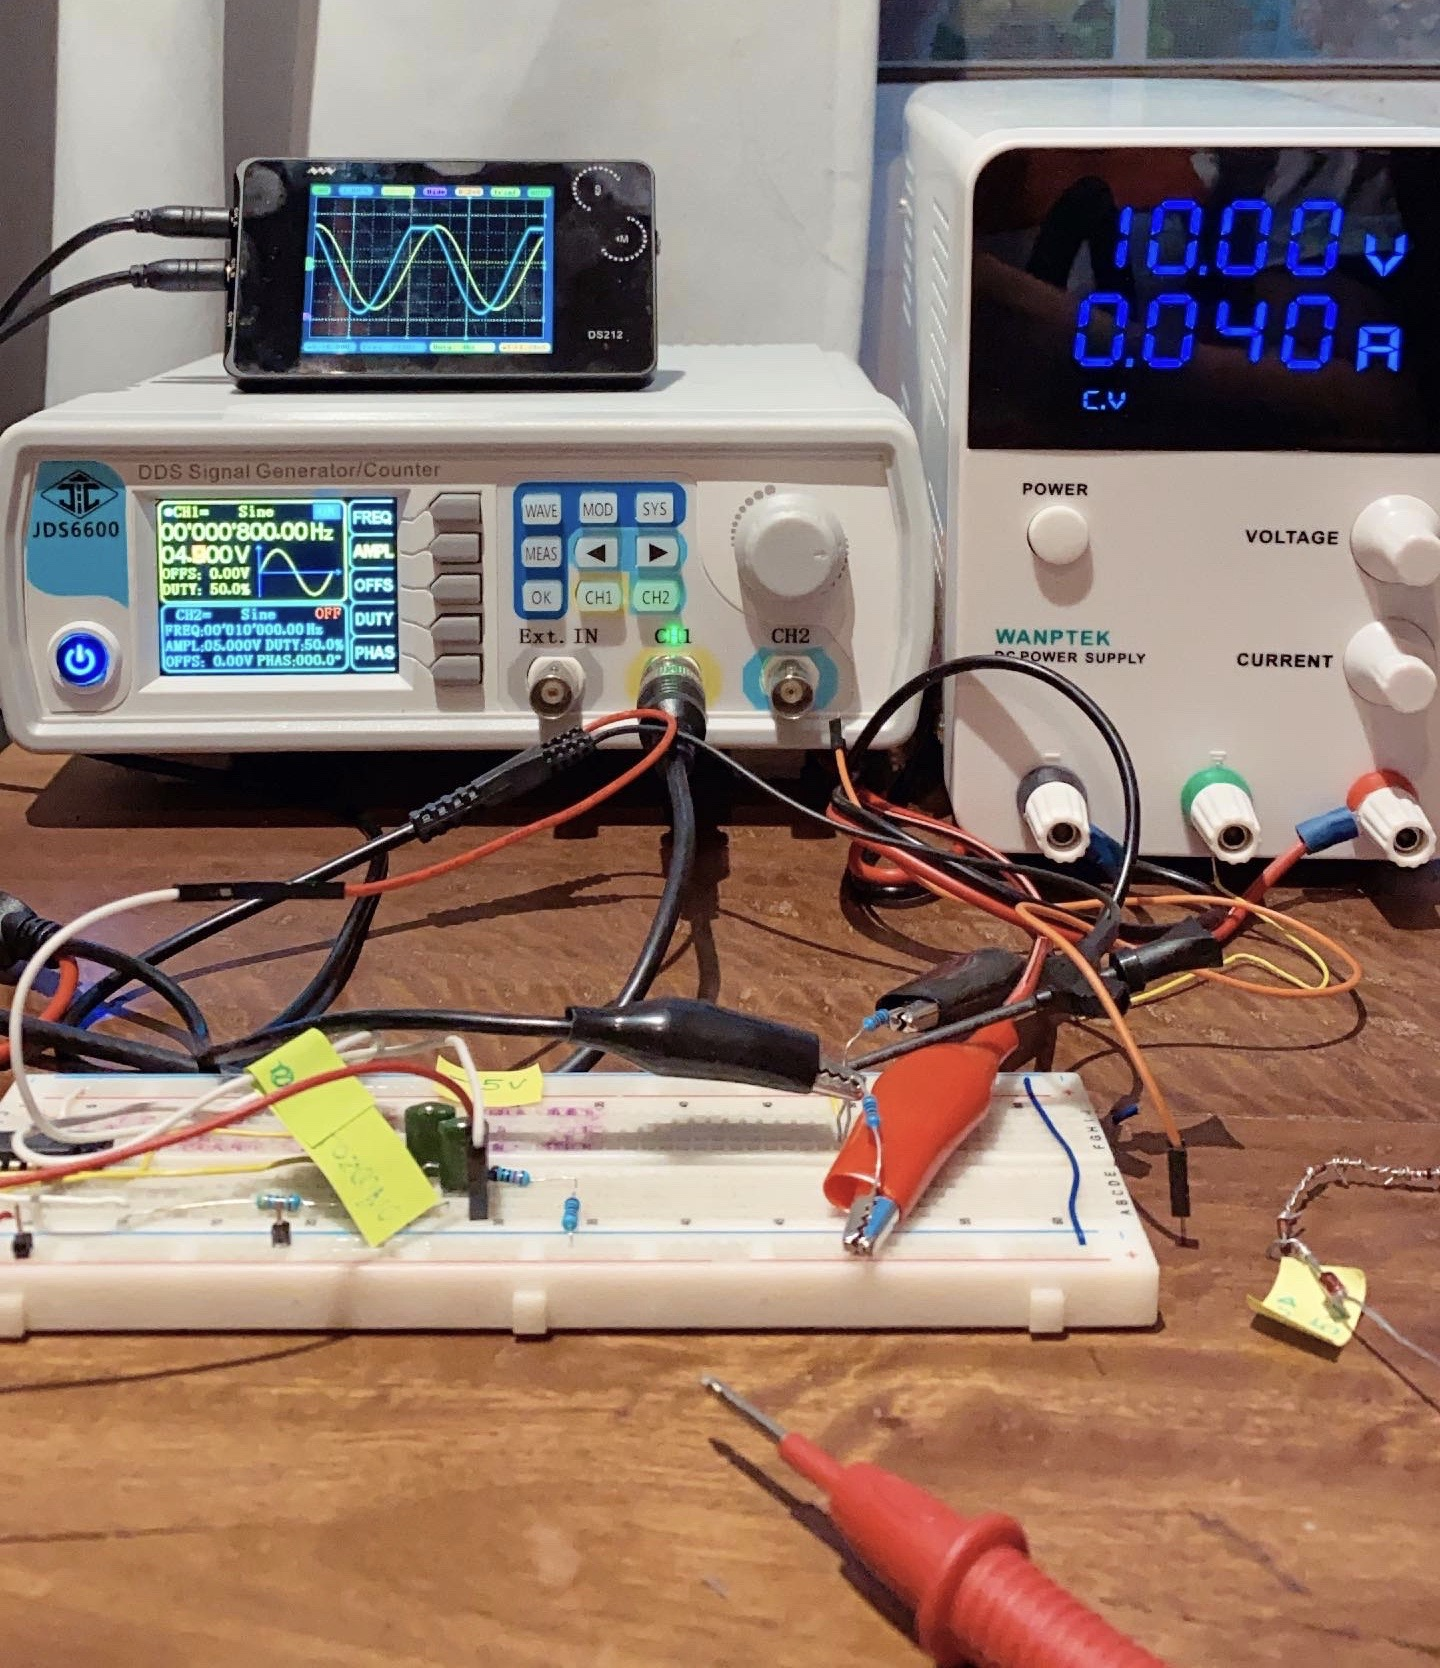
\includegraphics[width=7cm]{imagenes/BancoMedicion.JPG}	\caption{Banco de mediciones}	
\end{figure}
\end{centering}

\pagebreak

Luego de realizar las mediciones, se calcularon los valores de amplificacion en \dB\ y se confeccion\'o el siguiente diagrama

\begin{centering}
	\begin{figure}[h]
		\centering
		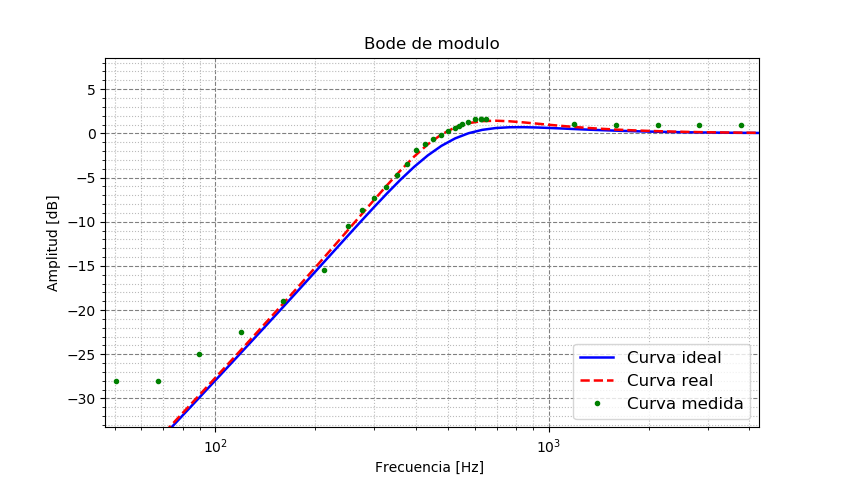
\includegraphics[width=0.8\textwidth]{imagenes/bodeMedicion}
		\caption{Diagrama de Bode para la medici\'on}
	\end{figure}
\end{centering}

Podemos apreciar que la curva formada por los puntos medidos se asimila mucho a la curva dada por la transferencia del circuito real, y es coherente que esta sea la que predice el funcionamiento del circuito dado que ese es su prop\'oito.\\
Haciendo un acercamiento sobre la zona de corte, podemos observar que hay m\'as cantidad de puntos y en esta zona, la similitud con la curva del circuito real es pr\'acticamente completa.

\begin{centering}
	\begin{figure}[h]
		\centering
		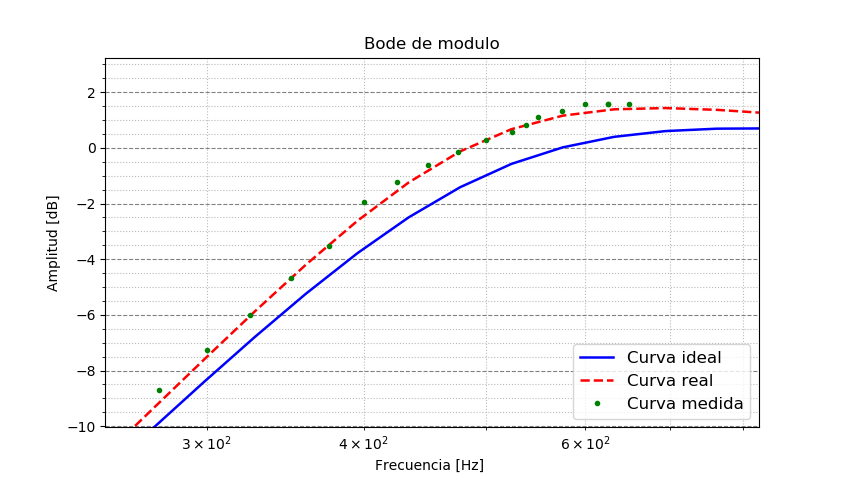
\includegraphics[width=0.8\textwidth]{imagenes/bodeMedicionDetalle.png}
		\caption{Vista en detalle de Bode para la medici\'on}
	\end{figure}
\end{centering}

\pagebreak

Luego, se defini\'o un procedimiento para medir la frecuencia de corte a $-3\dB$, y dado que lo observado en el osciloscopio son valores de tensi\'on, se encontr\'o el valor de tensi\'n a la salida del filtro tal que haya una amplificaci\'on de $-3\dB$, dada una tens\'on (amplitud) de entrada fija.
Siendo que la amplitud de entrada eran $3.1\V$, se busca que la amplitud a la salida sea de 
\begin{equation}
	V_0= 3,1 \V \ 10^{\frac{-3 \dB}{20}}	= 2.19\V
\end{equation}
Este nivel  de amplitud se encuentra en $f=390\Hz$, esto implica  una diferencia porcentual de $23\%$ con la frecuencia de corte.

Para el c\'alculo de las asintotas se tomaron los puntos antes y despu\'es de la frecuencia de corte donde existita una tendencia lineal, dado que la escala era semilogar\'itmica para el eje de las frecuencias, la relaci\'on lineal es de $log (f) \ vs\ A$ donde A es la amplificai\'on en \dB. Utilizando el metodo de \textit{Cuadrados m\'inimos} para la aproximaci\'on lineal, se encontraron las rectas $y_1=39.46x-105.48$ e $y_2=-0.24x+1.81$. Vemos a continuaci\'on el resultado de la regreci\'on lineal en el gr\'afico de Bode.

\begin{centering}
	\begin{figure}[h]
		\centering
		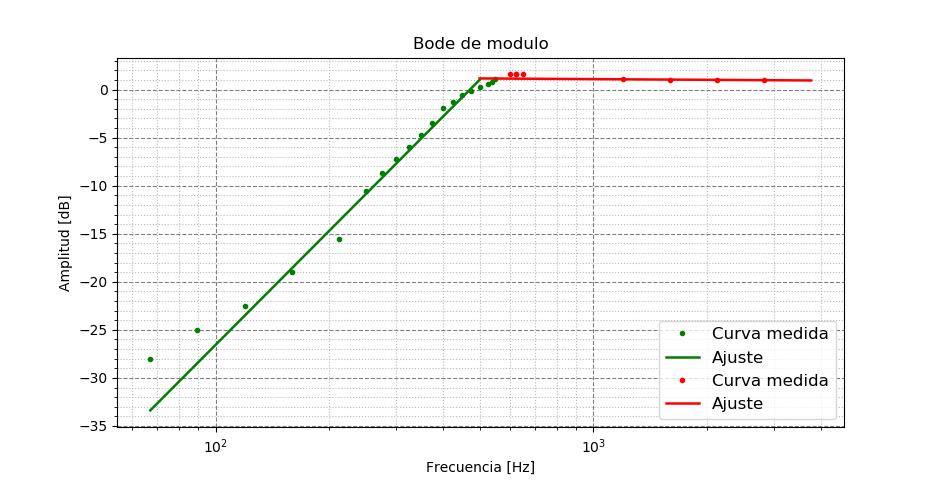
\includegraphics[width=0.6\textwidth]{imagenes/BodeMedicionAjuste.png}
		\caption{Ajuste lineal de Bode para la medici\'on}
	\end{figure}
\end{centering}

Viendo que las pendientes de las rectas dieron $a_1=39.46$ y $a_2=-0.24$, estos resultados son bastantes similares los valores esperados del desarrollo anal\'itico, esperandose valores de $40\dB$ y $0\dB$, los resultados encontrados supone una diferencia porcentual de $1.35\%$ para la primer pendiente, mientras que la diferencia de la segunda es atribuida al haber tomado puntos de la medici\'on donde todavia existia algun nivel de amplifiaci\'on.
Teniendo estos datos, se puede definir una frecuencia en la intersecci\'on de las rectas $y_1$ e $y_2$, esta di\'o un valor de $f=504,1 \Hz$, lo cu\'al implica un muy bajo error del $0.02\%$ 
\subsubsection*{Respuesta a excitaci\'on cuadrada}

Se realizaron 3 mediciones de respuesta a una señal cuadrada con las mismas especificaciones de la señal simulada anteriormente. Podremos observar en las siguientes imagenes, que los comportamientos generales son muy similares a los esperados, con las unicas diferencias siendo de caracteristicas propias de un circuito real, como el hecho de imposibilitar ganancia infinita por ejemplo.

\begin{centering}
	\begin{figure}[hbt]
		\centering
		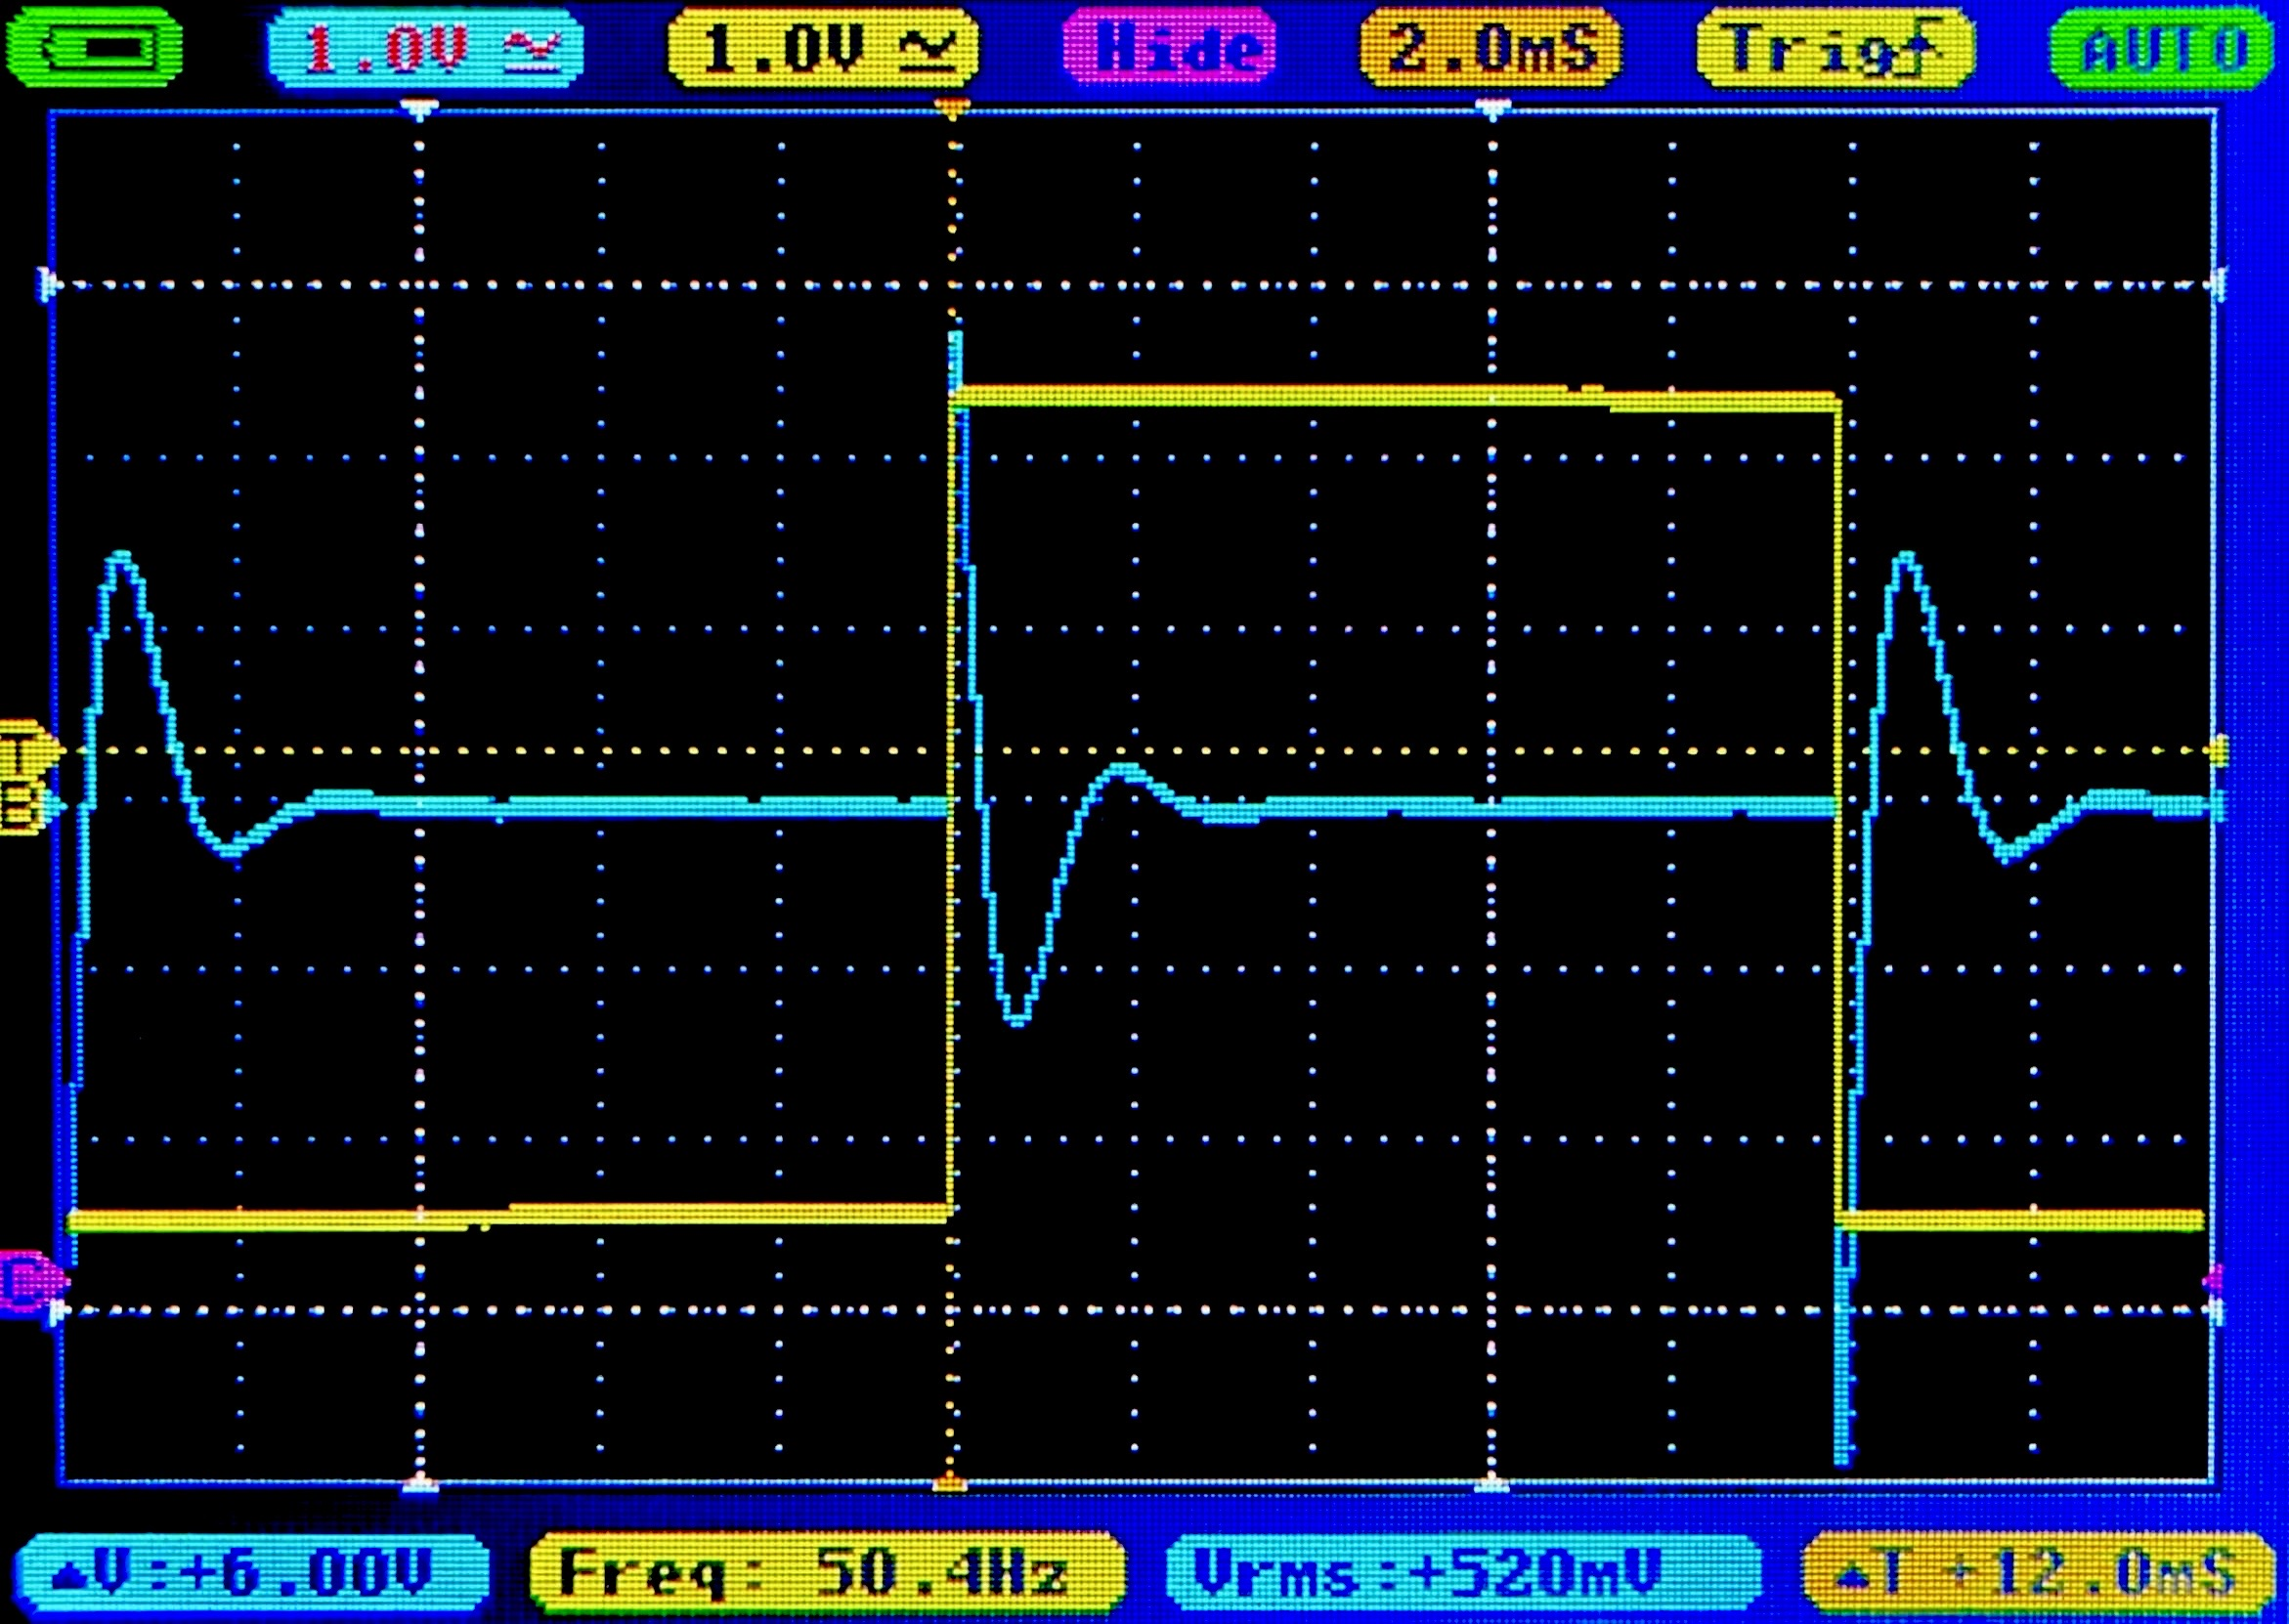
\includegraphics[width=0.4\textwidth]{imagenes/Captura50.JPG}
		\caption{Medici\'on en osciloscpio con una entrada cuadrada de 50.4 Hz}
	\end{figure}
\end{centering}

Se puede observar que la forma de la salida es muy similar a lo simulado, con la diferencia que los picos iniciales en cada flanco son mucho menores, pasando de tocar los $2\V$ a estar por debajo de los $1.5\V$. Las oscilaciones y otras caracteristicas se mantienen iguales a lo simulado.

\begin{centering}
	\begin{figure}[hbt]
		\centering
		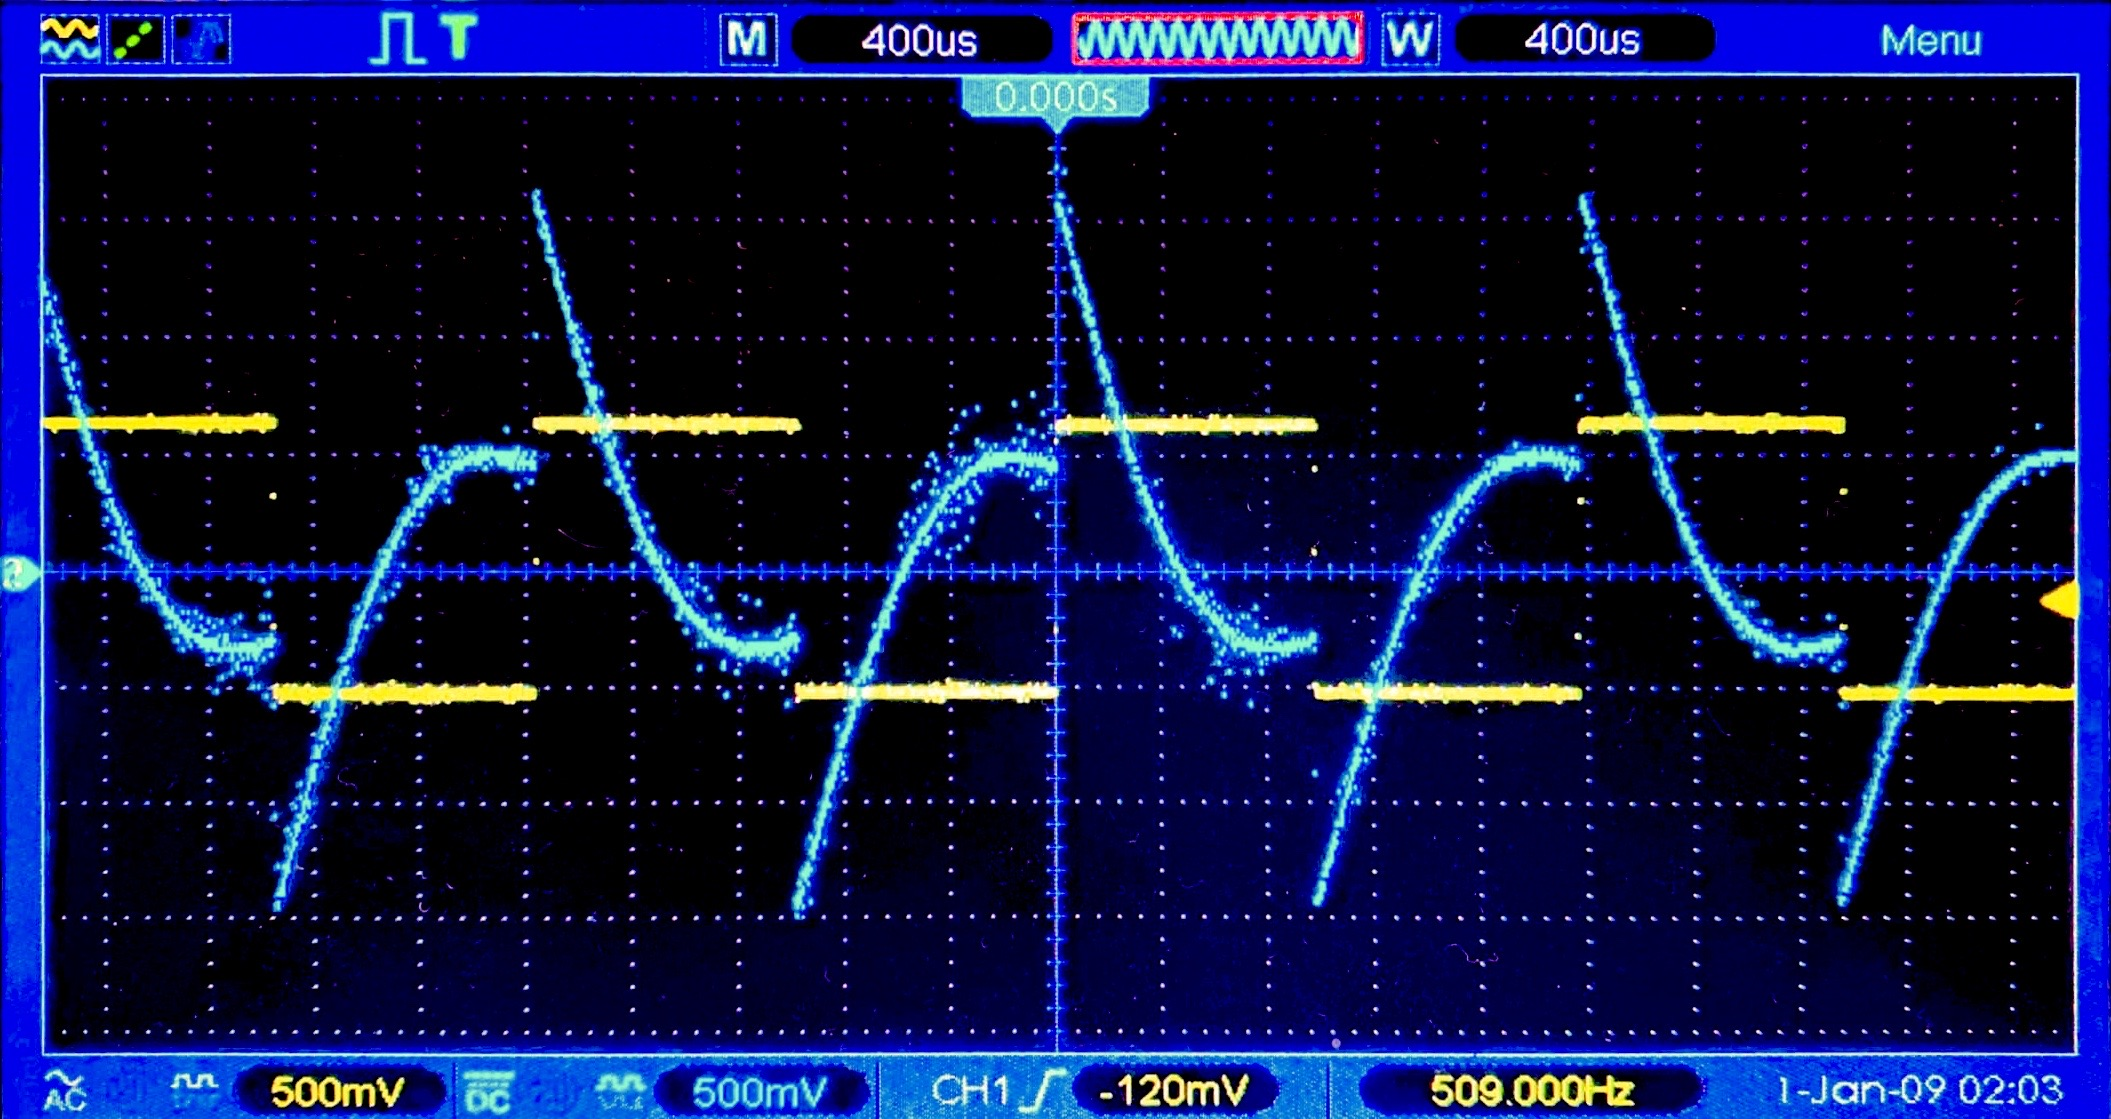
\includegraphics[width=0.4\textwidth]{imagenes/Captura500.JPG}
		\caption{Medici\'on en osciloscpio con una entrada cuadrada de 504 Hz}
	\end{figure}
\end{centering}

Nuevamente podemos observar que la forma  general se condice con lo visto en las simulaci\'ones y la diferencia vuelve a recaer en laamplitud del pico inicial de la salida, ahora teniendo un nivel maximo superior a lo simulado, donde previamente en la simulaci\'on se vieron picos que apenas superaban los $2.5 \V$, aqui vemos que llegan comodamente a los $3 \V$. Analizando el resto de la onda, aqui tampoco se observan oscilaciones como en la simulaci\'on,  donde el semiciclo de la entrada finaliza antes de que se estas formen.

\begin{centering}
	\begin{figure}[hbt]
		\centering
		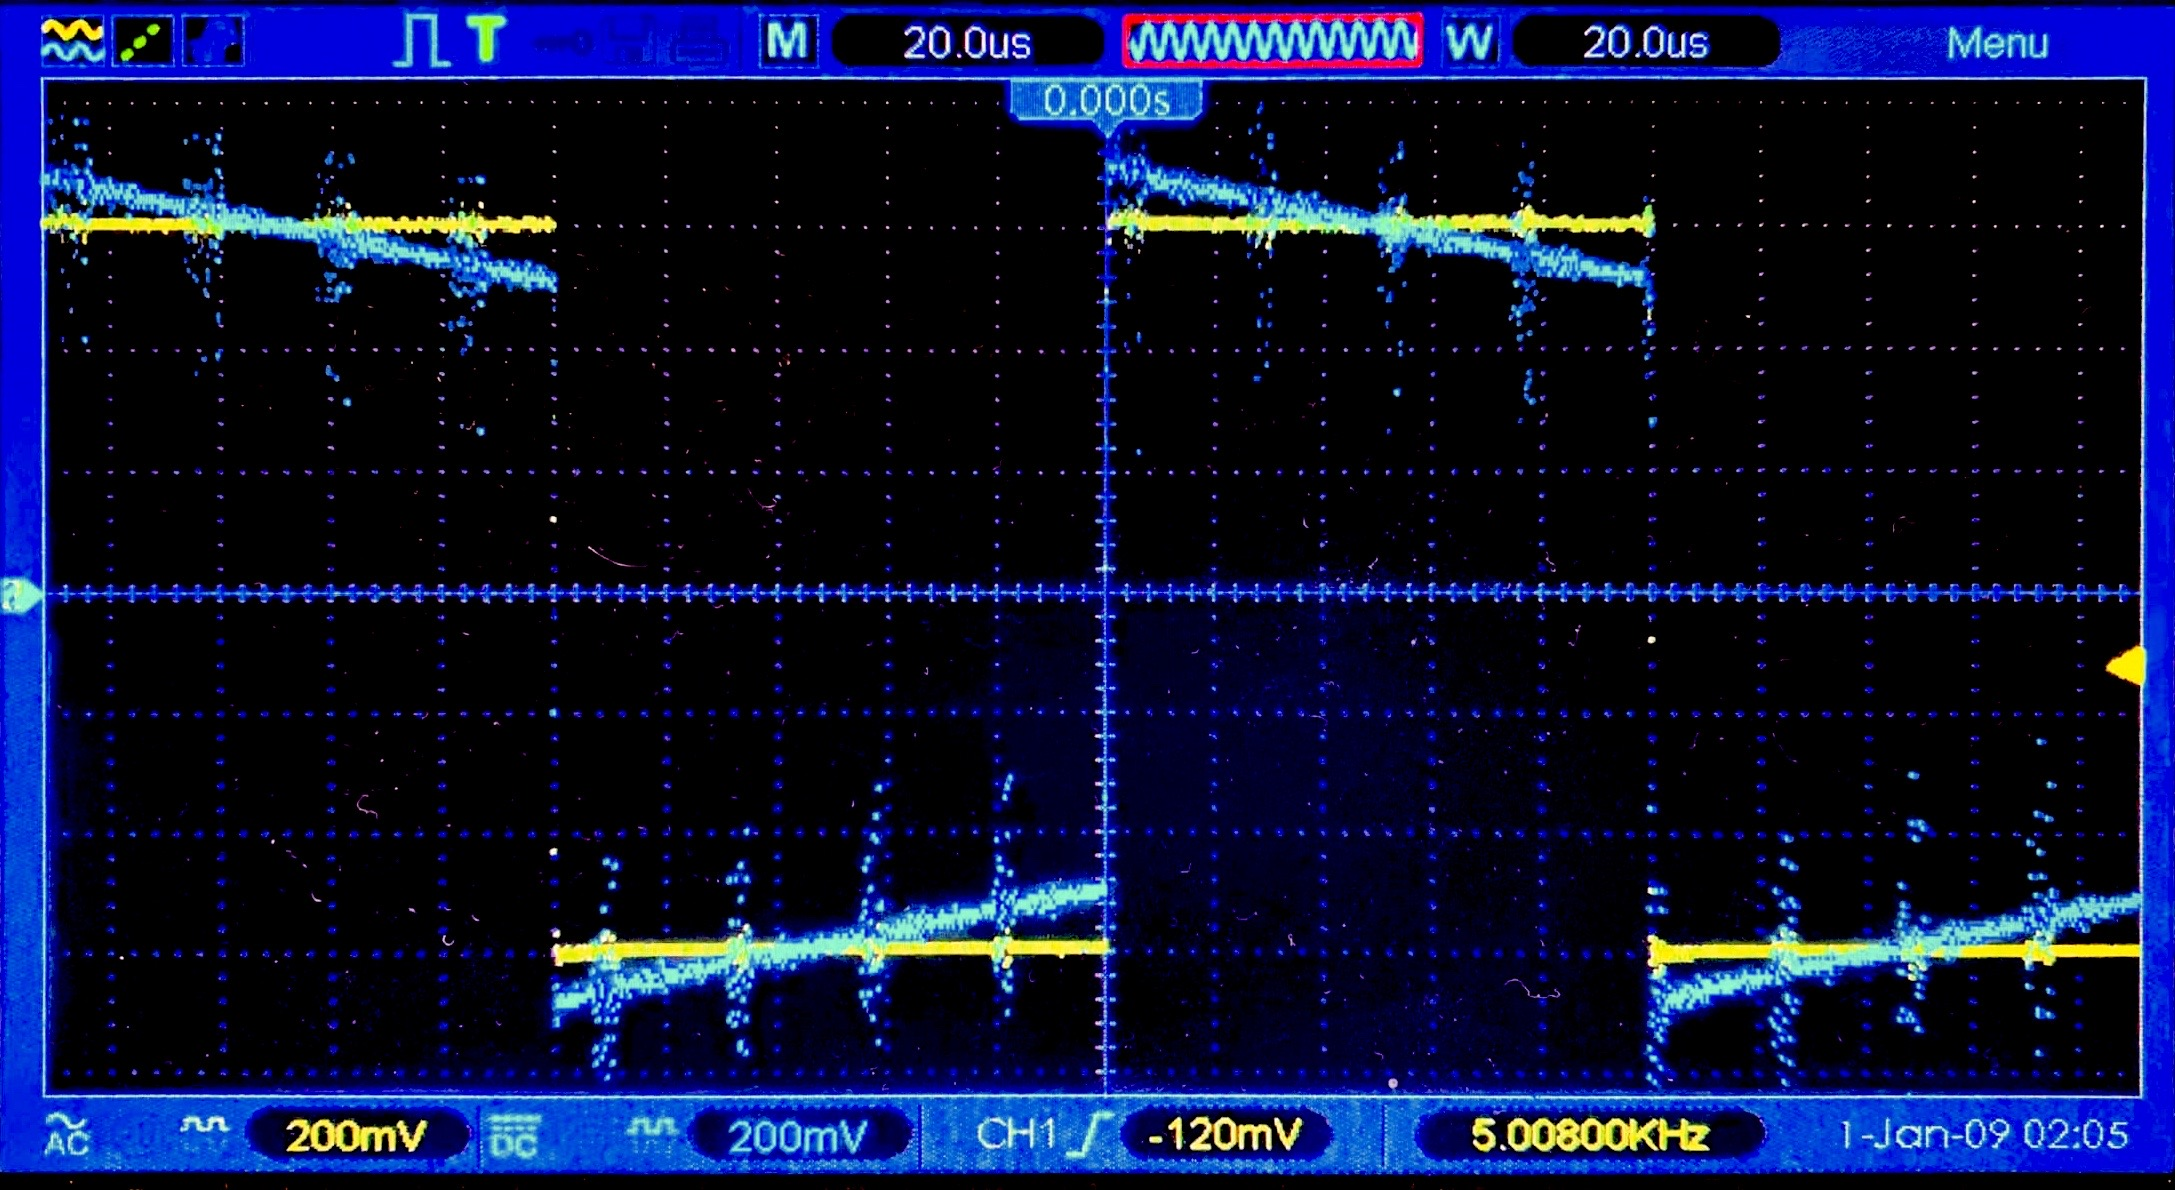
\includegraphics[width=0.4\textwidth]{imagenes/Captura5000.JPG}
		\caption{Medici\'on en osciloscpio con una entrada cuadrada de 5040 Hz}
	\end{figure}
\end{centering}

Por \'ultimo en la salida de mayor frecuencia, vemos que el comportamiento del filtro es practicamente igual al de la simulaci\'on, tambien podemos  observar que existe un ruido en el generador que esta siendo amplificado por el filtro, esto puede ser debido a las bajas prestaciones del generador de funciones o debido a un ruido interno del aparato. No causa mayores dificultades para este an\'alisis.
\pagebreak
%---------------------------------------------------------------%
